\subsection{Comparação visual de rotas por família}
Para cada família (C, R e RC), foi selecionada uma instância por critério combinado: maior melhoria de custo em relação ao I1 e maior proximidade do melhor valor conhecido (BKS).
Essa visualização padroniza a comparação qualitativa: a mesma instância é observada sob os cinco algoritmos.

\begin{figure}[htbp]
\centering
\IfFileExists{figs/png/route_compare_C.png}{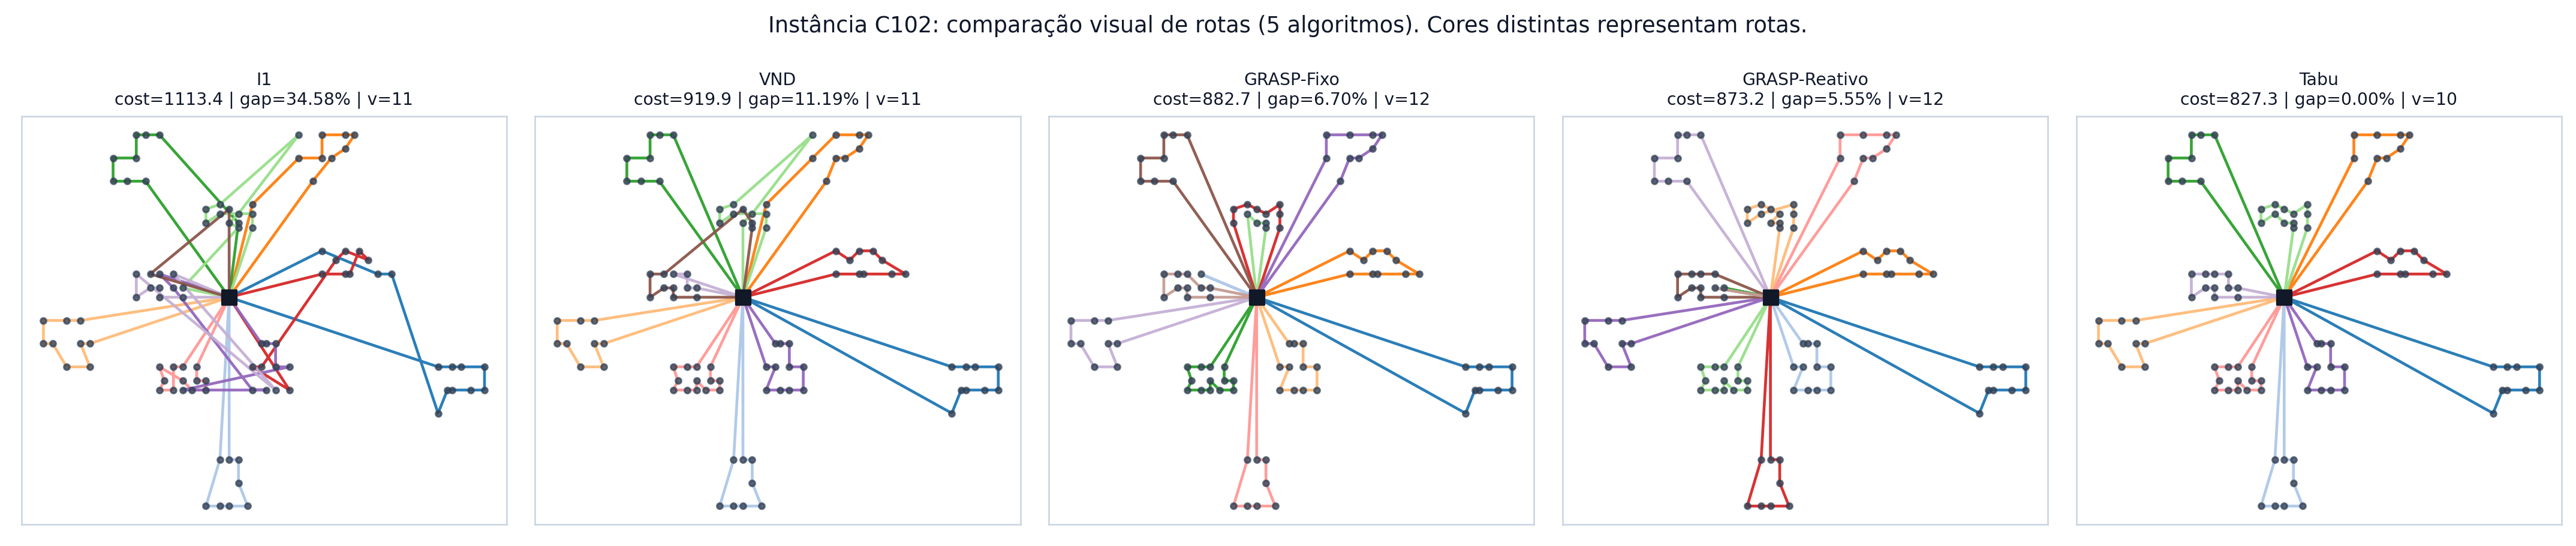
\includegraphics[width=\linewidth]{figs/png/route_compare_C.png}}{\fbox{\parbox{0.9\linewidth}{Figura ausente. Execute \texttt{python3 scripts/build_article_route_panels.py}.}}}
\caption{Família C: instância C102 (ganho vs I1 = 286.1, 25.70\%; distância ao BKS do melhor método = 0.0). Melhor algoritmo nessa instância: \texttt{tabu}. Cada coluna mostra a rota final de um algoritmo na mesma instância.}
\label{fig:route_compare_C}
\end{figure}

\begin{figure}[htbp]
\centering
\IfFileExists{figs/png/route_compare_R.png}{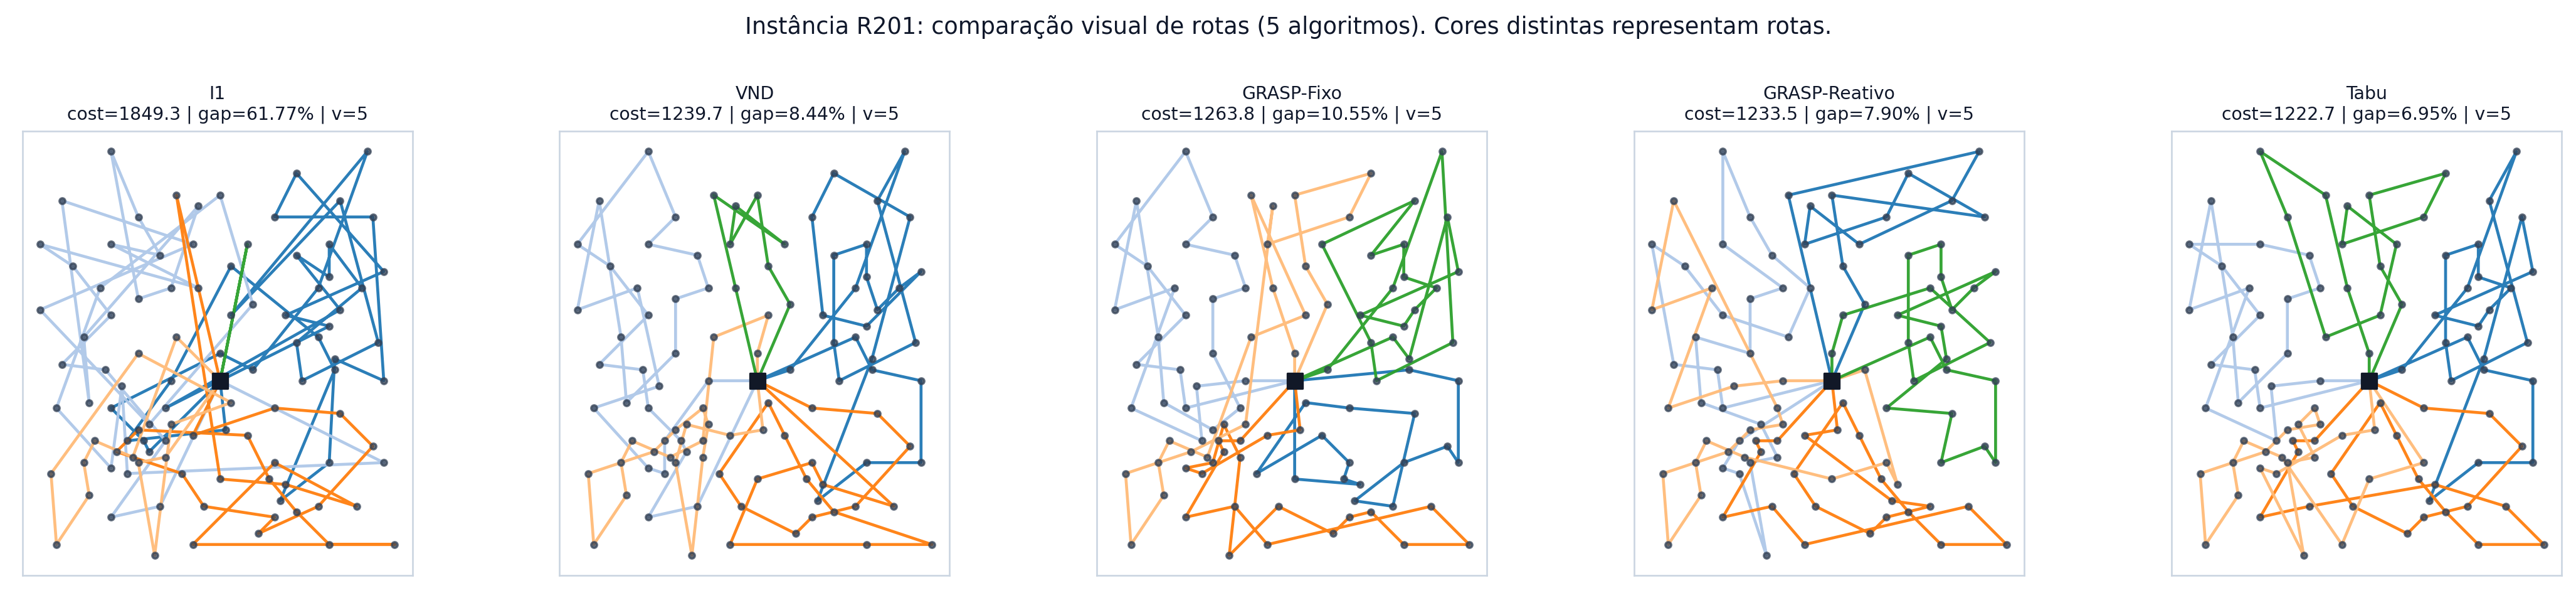
\includegraphics[width=\linewidth]{figs/png/route_compare_R.png}}{\fbox{\parbox{0.9\linewidth}{Figura ausente. Execute \texttt{python3 scripts/build_article_route_panels.py}.}}}
\caption{Família R: instância R201 (ganho vs I1 = 626.6, 33.88\%; distância ao BKS do melhor método = 79.5). Melhor algoritmo nessa instância: \texttt{tabu}. Cada coluna mostra a rota final de um algoritmo na mesma instância.}
\label{fig:route_compare_R}
\end{figure}

\begin{figure}[htbp]
\centering
\IfFileExists{figs/png/route_compare_RC.png}{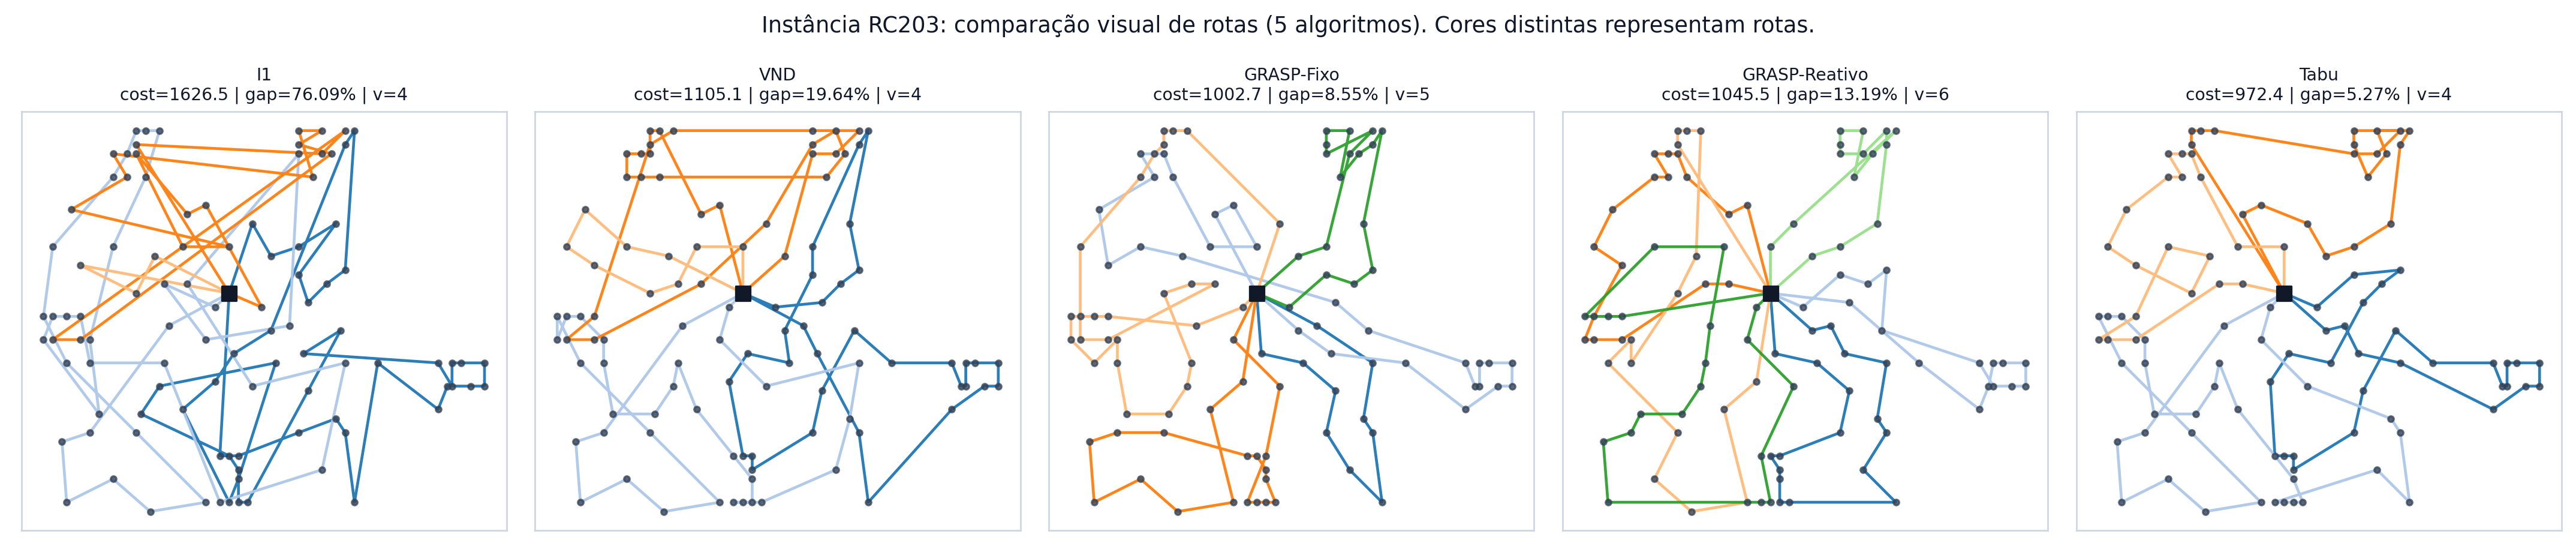
\includegraphics[width=\linewidth]{figs/png/route_compare_RC.png}}{\fbox{\parbox{0.9\linewidth}{Figura ausente. Execute \texttt{python3 scripts/build_article_route_panels.py}.}}}
\caption{Família RC: instância RC203 (ganho vs I1 = 654.1, 40.22\%; distância ao BKS do melhor método = 48.7). Melhor algoritmo nessa instância: \texttt{tabu}. Cada coluna mostra a rota final de um algoritmo na mesma instância.}
\label{fig:route_compare_RC}
\end{figure}
